Nous effectuons chaque jour certaines actions plutôt que d'autres : "si je suis debout tôt, alors je vais chercher le petit déjeuner". En informatique, il est possible de faire raisonner une ordinateur d'une manière assez similaire\footnote{Pour les conditions hein, pas pour le petit déjeuner !}. % je suis mdr

Typiquement, les programmes informatiques utilisent des expressions dont on évalue la valeur selon certains opérateurs pour savoir si elle vaut \textbf{True} ou \textbf{False}.

L'action effectuée par l'ordinateur sera différente en fonction de la valeur (True ou False) de l'expression.

\subsection{Outils de comparaison}
Voici les opérations de comparaison disponibles en \textsc{Python} :

\begin{table}[!h]
    \centering
    \begin{tabular}{|c|c|}
        \hline
         Opération & Description\\
        \hline
        $==$ & Egalité \\
        \hline
        $!=$ & Différent \\
        \hline
        $>$ & Plus grand \\
        \hline
        $>=$ & Plus grand ou égal \\
        \hline
        $<$ & Plus petit  \\
        \hline
        $<=$  & Plus petit ou égal \\
        \hline
    \end{tabular}
    \caption{Comparaison}
    \label{operStr}
\end{table}

\begin{python}[caption = Quelques comparaisons en python]
a = 5 > 4 # a vaut True
b = 0.5 >= 1 # b vaut False
c = 1 > "salut" # Que se passe t il ?
\end{python}

\subsection{Opérateurs logiques}
Ce n'est pas tout ! On peut encore combiner ces expressions avec des opérateurs logiques.

Typiquement,on pourrait vouloir que deux conditions soient respectées, qu'au moins l’une des deux soit respectée ou qu'une condition ne soit pas respectée. Ceci est possible via les opérateurs \textsc{et}, \textsc{ou} et \textsc{non}. 
\paragraph{Table logique}
Chaque opérateur logique peut être défini par une table logique :

\begin{table}[!h]
    \begin{tabular}{cp{1cm}cp{1cm}c}
            \begin{tabular}{c|cc}
                \diaghead{\theadfont bbbbbbb}{a}{b}
                & \texttt{True} & \texttt{False} \\
                \hline
                \texttt{True} & \texttt{True} & \texttt{True} \\
                \texttt{False} & \texttt{True} & \texttt{False} \\
            \end{tabular}
            & &
            \begin{tabular}{c|cc}
                \diaghead{\theadfont bbbbbbb}{a}{b}
                & \texttt{True} & \texttt{False} \\
                \hline
                \texttt{True} & \texttt{True} & \texttt{False} \\
                \texttt{False} & \texttt{False} & \texttt{False} \\
            \end{tabular}
            & &
            \begin{tabular}{c|c}
                a & \\
                \hline
                \texttt{True} & \texttt{False} \\
                \texttt{False} & \texttt{True} \\
            \end{tabular}
            \\
            &&&& \\

            (a) OU & & (b) ET & & (c) NON \\
    \end{tabular}
    \caption{Table logique des opérateurs logiques}
\end{table}

\paragraph{En python}
En \textsc{python}, les opérateurs sont représentés à l'aide de
\texttt{and, or, not}.

\begin{table}[!h]
    \centering
    \begin{tabular}{|c|c|}
        \hline
        a OU b & a or b\\
        \hline
        a ET b & a and b \\
        \hline
        NON a & not a \\
        \hline
    \end{tabular}
    \caption{Opérateurs logiques en \textsc{Python}}
\end{table}

\subsubsection{Combinaisons}
Les opérateurs logiques ainsi expressions conditionnelles peuvent être combinés à l'infini pour former des expressions plus complexes. Cependant, comme pour les opérations mathématiques, il existe un ordre de priorité : d'abord \texttt{not}, puis \texttt{and}, puis \texttt{or}. Pour éviter les ambiguïtés et améliorer la lisibilité d'une expression complexe, on peut (et c'est conseillé!) y mettre des parenthèses.

\begin{python}[caption = Expressions booléennes]
a = True
b = False
c = a or b #c est vrai
d = a and b #d est faux
e = not b and a #e est vrai
f = (not (a and b)) or (not ((not d) and (a or e))) #f vaut True
\end{python}
\textbf{Exercices : } Evaluez les expressions suivantes :
\begin{python}[caption = Exercices d'expressions booléennes]
bool_one = False or not True and True
bool_two = False and not True or True
bool_three = True and not (False or False)
bool_four = not not True or False or not True
bool_five = False or not (True and True)
\end{python}
\subsubsection{Le \texttt{if}}
On peut représenter l'ensemble des exécutions possibles d'un programme comme un arbre de décision. Selon la valeur de certaines expressions, l'exécution du programme va prendre une direction ou
l'autre...


En résumé, certaines parties du code sont exécutées sous
certaines conditions!

\begin{figure}[!h]
    \centering
    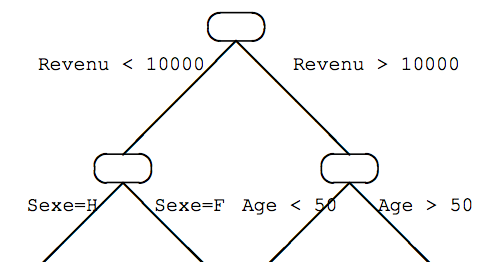
\includegraphics[width=7cm]{img/arbre.png}
    \caption{Arbre binaire de décision}
    \label{arbre}
\end{figure}

Afin de représenter ce choix, \textsc{Python} contient la clause \texttt{if} suivi d'une une expression booléenne et de \texttt{:}. Si la condition est vraie, le programme exécute toutes les instructions \textit{indentées}\footnote{Une expression indentée est une expression précédée d'une tabulation} qui suivent. Dans le cas contraire, ces instructions ne sont pas exécutées.

\begin{python}[caption = l'instruction if]
a = 10
if a > 5:
    print("Cette instruction est executee")
print("fin du code")
\end{python}
Il est aussi possible de donner un choix alternatif grâce à l'instruction \texttt{else:}. Si l'expression dans le \texttt{if} est \texttt{False}, le programme exécute alors le code \textit{indenté} qui suit le \texttt{else}.
\begin{python}
a = 10
if a < 5:
    print("Cette instruction n'est pas executee")
else:
    print("Cette instruction est executee")
print("fin du code")
\end{python}

\subsection{Le \texttt{elif}}
Vous pouvez construire des clauses \texttt{if} plus complexes en rajoutant des \texttt{elif}. Attention, à la première condition vraie rencontrée, on quitte la condition! Les expressions suivantes ne sont même pas évaluées.

\begin{python}[caption = utilisation de elif]
x = 200
if x > 10:
    print("A")
elif x > 100:
    print("B")
else:
    print("C")
# Seul 'A' est imprime, pas 'B' !!!
\end{python}
La clause \textbf{elif} permet d'augmenter l'embranchement 
(c'est-à-dire le nombre de choix possibles) de notre arbre de décisions!

\subsection{Code mort}

Lorsque vous utilisez des conditions, faites attention à ne pas créer du \textit{code mort}, c'est-à-dire du code qui ne sera jamais exécuté.
\begin{python}[caption = Exemple de code mort]
if False:
    print("Ce code n'est jamais execute!")
\end{python}

\subsection{Exercice}
Écrivez un code qui demande à l'utilisateur d'entrer un chiffre et imprime "Félicitations, votre chiffre est un multiple de 7" si le chiffre est divisible par 7. Et "Désolé, votre chiffre n'est pas un multiple de 7" sinon.
